

\documentclass[10pt, titlepage, oneside, a4paper]{article}
\usepackage[T1]{fontenc}
\usepackage[utf8]{inputenc}
\usepackage[swedish]{babel}
\usepackage{amssymb, graphicx, fancyhdr}
\usepackage{hyperref}
\addtolength{\textheight}{20mm}
\addtolength{\voffset}{-5mm}
\renewcommand{\sectionmark}[1]{\markleft{#1}}

\newcommand{\Section}[1]{\section{#1}\vspace{-8pt}}
\newcommand{\Subsection}[1]{\vspace{-4pt}\subsection{#1}\vspace{-8pt}}
\newcommand{\Subsubsection}[1]{\vspace{-4pt}\subsubsection{#1}\vspace{-8pt}}
	


\def\typeofdoc{Laborationsrapport}
\def\course{D0036D}
\def\pretitle{Laboration 3}
\def\title{JavaGameServer \& Client}
\def\name{Magnus Björk}
\def\username{magbjr-3}
\def\email{\username{}@student.ltu.se}
\def\graders{Örjan Tjernström}
\def\university{Luleå Tekniska Universitet}


\def\fullpath{\raisebox{1pt}{$\scriptstyle \sim$}\username/\path}


\begin{document}
	\begin{titlepage}
		\thispagestyle{empty}
		\begin{large}
			\begin{tabular}{@{}p{\textwidth}@{}}
				\textbf{\university \hfill \today} \\
				\textbf{\typeofdoc} \\
			\end{tabular}
		\end{large}
		\vspace{10mm}
		\begin{center}
			\LARGE{\pretitle} \\
			\huge{\textbf{\course}}\\
			\vspace{10mm}
			\LARGE{\title} \\
			\vspace{15mm}
			\begin{large}
				\begin{tabular}{ll}
					\textbf{Namn} & \name \\
					\textbf{E-mail} & \texttt{\email} \\
				\end{tabular}
			\end{large}
			\vfill
			\large{\textbf{Handledare}}\\
			\mbox{\large{\graders}}
		\end{center}
	\end{titlepage}

	\lfoot{\footnotesize{\name, \email}}
	\rfoot{\footnotesize{\today}}
	\lhead{\sc\footnotesize\title}
	\rhead{\nouppercase{\sc\footnotesize\leftmark}}
	\pagestyle{fancy}
	\renewcommand{\headrulewidth}{0.2pt}
	\renewcommand{\footrulewidth}{0.2pt}

	\pagenumbering{roman}
    \tableofcontents
	
	\newpage

	\pagenumbering{arabic}

	\setlength{\parindent}{0pt}
	\setlength{\parskip}{10pt}

	\section{Introduktion}
		Laborationsuppgiften var att programmera ett nätverksspel. Syftet med uppgiften var att man skulle utvidga sin kunskap gällande:
		
        \begin{itemize}
        	\item \textbf{Nätverksprotokoll} 
        		\begin{itemize}
        			\item \textbf{TCP} \\ Pålitligt protokoll för dataöverföring. Lämpligt att använda vid viktiga tillfällen i spelet. \textit{T.ex. när en klient ansluter eller lämnar en server.}
        			\item \textbf{UDP} \\ Opålitligt men snabbt protokoll för dataöverföring. Snabbare än TCP på grund av att det dels inte skickar tillbaka något ACK-meddelande till sändaren samt att UDP har en mindre 'frame'. Lämpar sig bäst för uppdateringar av förflyttningar på grund av sin snabbhet.
        		\end{itemize}
            \item \textbf{Sockets} \\
            Spelet skulle innehålla kommunikation över nätverket, detta sköts av diverse sockets:
            	\begin{itemize}
            		\item \textbf{DatagramSocket} \\Hanterar trafik av protokollet UDP. Kan skicka unicast till en annan DatagramSocket eller multicast genom att skicka till en multicast-grupp. \textit{T.ex. Önskemål om förflyttning från klient till server.}
            		
            		\item \textbf{MulticastSocket} \\Hanterar inkommande multicast-trafik av protokollet UDP. En MulticastSocket går med i en multicast-grupp för att få ta del av dess trafik. \textit{T.ex. uppdateringar av spelarnas position från server till klienter.)}
            		\item \textbf{ServerSocket} \\Serversocket tar emot trafik av protokollet TCP. Ansluter en klient till servern kan man sedan skapa ett Socket objekt för att hantera strömmen.
            		\item \textbf{Socket} \\ Hanterar TCP-trafik. Skapas av ServerSocket på server-sidan. Klienten skapar den socket som tar kontakt med servern.
            		
            	\end{itemize}
          	
			\item \textbf{Trådning} \\En del moment måste köras parallellt och då kan man använda trådar. \textit{T.ex. så har varje klient en tråd på servern som den kommunicerar med.}
        \end{itemize}
        \newpage
        
	\section{Metod}
	
		Min strategi för att lösa uppgiften var att dela upp koden i 3 lager. Detta för att göra det enkelt att lägga på funktioner. \textit{T.ex. Uppgiften att flytta uppdateringsmeddellanden från TCP till UDP var relativt smärtfri, hade spelmekanik varit inblandad i denna del hade det varit betydligt värre.}
		\begin{itemize}
			\item \textbf{Nätverk} Nätverkskoden skall endast skicka meddellanden mellan servern och klienten. Ingenting som har med spel-lagret att göra skall finnas här.
			\item \textbf{Spel} Spelets logik och utseende skall endast påverkas av kommunikations-lagret av programmet.
			\item \textbf{Kommunikation}\\Det lager som sköter kommunikation mellan Spel- och Nätverks-lagren. 
		\end{itemize}
		
		\subsection{Design}
			\begin{center}
				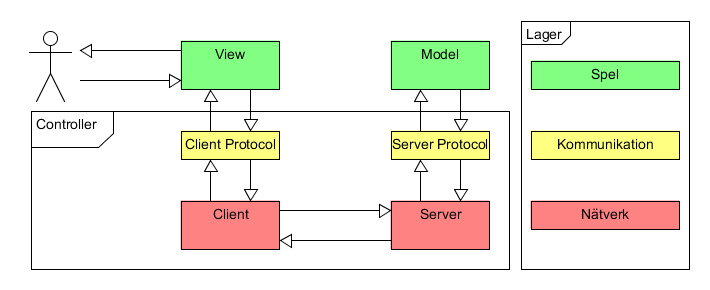
\includegraphics[scale=.5]{./documentation/images/abstract.png}
			\end{center}
			
			Jag ville skapa ett dataflöde liknande bilden ovan.
			\begin{enumerate}
				\item Spelaren trycker på en tangent för att flytta sin markör.
				\item Klient-protokollet skapar ett meddelande med användarens indata och skickar detta till nätverkslagret.
				\item Nätverkslagret skickar nu meddelandet från klienten till servern.
				\item Server-protokollet tar emot och bearbetar modellen efter anvisningar i meddelandet. Skapar ett nytt meddelande som skickas tillbaka till klienten via nätverkslagret.
				\item Klient-protokollet tar emot meddelandet och ändrar eventuellt vyn som visas för spelaren.
				\item Spelaren upptäcker förflyttningen (Om den var giltig) och kan nu ge ny indata om den så vill.
			\end{enumerate}
		
	\section{Resultat}
		\subsection{Användarhandledning}
		
		\subsection{Handskakning}
		\subsection{Applikationsprotokoll}
			\subsubsection{Klient}
			\subsubsection{Server}
	\section{Diskussion}
		\subsection{Synchronize}
    
    
\end{document}
